\documentclass[12pt,oneside]{book}

% Маргине, проред и тако то
\usepackage[a4paper, margin=30mm]{geometry}
\renewcommand{\baselinestretch}{1.5}

% Фонтови, енкодинг
\usepackage[]{mathtext}
\usepackage[T2A, TS1]{fontenc}
\usepackage[utf8]{inputenc}
\usepackage[english, russian, serbianc]{babel}
%\usepackage[russian]{babel}
\usepackage{babelbib}

\usepackage{graphicx}
\DeclareGraphicsExtensions{.pdf,.png,.jpg}
\usepackage{tikz}

\usepackage[cmex10]{amsmath}
\usepackage{amssymb}

\usepackage[caption=false,font=footnotesize]{subfig}
\renewcommand{\thesubfigure}{\asbuk{subfigure}}

\usepackage{siunitx}
\sisetup{detect-all = true,
range-phrase = --,
range-units = single,
output-decimal-marker = {,}}
\usepackage{physics}
\usepackage{nicefrac}

%\usepackage[usenames,dvipsnames,svgnames,table]{xcolor}
%\usepackage{soul}
%%\definecolor{lightblue}{rgb}{.90,.95,1}
%\colorlet{lightblue}{cyan!50}
%\sethlcolor{lightblue}

%\usepackage[nomarkers]{endfloat}%notablist,nofiglist ili nolists

\usepackage[]{foreign}

\title{АСИМЕТРИЧНИ РЕЗОНАТОРИ КАО ЕЛЕМЕНТИ ЈЕДИНИЧНИХ ЋЕЛИЈА ЈЕДНОДИМЕНЗИОНАЛНИХ МЕТАМАТЕРИЈАЛА}
\date{\today}
\author{Војислав Милошевић}

\begin{document}

\chapter{Увод}

\tableofcontents

\section{Основни појмови}

Метаматеријали се могу дефинисати као вештачке композитне структуре, које поседују необичне особине, које је тешко, или немогуће, наћи у природи~\cite{Sham:09}. Очигледно је оваква дефиниција веома општа, међутим, услед велике разноврсности у самој области, као и непостојања консензуса у литератури, тешко је дати прецизнију свеобухватну дефиницију. У наставку ће бити дат преглед области...% хм... некако би требало ово мало преправити

Особине метаматеријала од интереса готово искључиво су везане за њихову интеракцију са различитим типовима таласа. Најчешће, у питању су електромагнетни (ЕМ) таласи, у ком случају се говори о ЕМ метаматеријалима, мада постоје и други типови (нпр. акустички). У овој тези ће се говорити искључиво о ЕМ метаматеријалима, што се у даљем тексту неће посебно наглашавати.

Метаматеријали се обично реализују као периодичне структуре са резонантним елементима, при чему периодичност може бити у једној, две или три димензије. Претпоставка је да је период, $d$, много мањи од таласне дужине, $\lambda$, у опсегу од интереса (обично у околини резонансе елемената), тако да се метаматеријал понаша као континуална средина~\cite{landau1982}. У том случају се може извршити хомогенизација Максвелових једначина, при чему се материјал описује \emph{ефективним параметрима}, као што су диелектричка пермитивност, $\varepsilon$, магнетна пермеабилност, $\mu$. Разлика у односу на фотонске кристале, који су такође периодичне структуре, дефинише се преко односа $\frac{d}{\lambda}$; уколико је он мањи од $\frac{1}{2}$, што одговара првој Браговој резонанси, ради се о режиму метаматеријала. За већину метаматеријала приказаних у литератури овај однос је приближно око $\frac{1}{4}$. С обзиром да је овај однос много већи него што је обично случај за природне материјале, хомогенизација метаматеријала је предмет одређених контроверзи~\cite{simovski}.

Микроталасна техника се бави пројектовањем кола, компонената и система који раде на учестаностима условно од \SI{300}{\mega\hertz} до \SI{300}{\giga\hertz} (односно таласне дужине од \SI{1}{\meter} до \SI{1}{\milli\meter}). Прецизнији опис је да се ради о колима чије димензије су упоредиве са таласном дужином сигнала, што има битне последице на начин рада и пројектовање. На пример, за пренос сигнала морају се користити водови или таласоводи, чије особине битно утичу на остатак кола, за разлику од нижих учестаности, где се сигнал преноси било каквим електричним контактом, чији утицај се може занемарити. Најважније примене микроталасне технике су најпре радарски системи и телекомуникације, који раде на овим учестаностима због широког опсега и повољних услова простирања, и довољно мале таласне дужине да се могу направити усмерене антене. Такође, многе атомске и молекуларне резонансе од интереса налазе у микроталасном опсегу, због чега постоје примене у радио-астрономији, медицини, даљинској детекцији (\foreign{remote sensing})~\cite{djordjevic2005mikrotalasna,pozar2009microwave}.  \cite{markes_knjiga}

\section{Особине средине са истовремено негативним параметрима $\varepsilon$ и $\mu$}
\subsection{Простирање таласа}

Очекивано је да реални делови пермитивности, $\varepsilon$, и пермеабилности, $\mu$, буду позитивни – ово произилази из једноставне чињенице да се елементарна наелектрисања и магнетни моменти у материјалу оријентишу у смеру спољашњег поља. Ипак, ако се посматрају временски променљива поља, мора се узети у обзир дисперзија параметара, $\varepsilon(\omega)$ и $\mu(\omega)$; и могуће је да постоје негативне вредности на одређеним фреквенцијама. Многи материјали у природи испољавају $\varepsilon < 0$, нпр. плазма испод Друдеове учестаности. Материјали са $\mu<0$ су ретки, али ово својство испољавају нпр. ферити на микроталасним учестаностима. Ипак, све до недавно нису били познати материјали код којих би истовремено важило $\varepsilon,\mu < 0$.

У свом познатом раду, Веселаго је хипотетички разматрао постојање таквог материјала~\cite{veselago_cir}. У изотропној средини, из Максвелових једначина може се извести скаларни облик таласне једначине:
\begin{equation}
    \left( \nabla^2 - \frac{n^2}{c^2}\frac{\partial}{\partial t} \right) \psi = 0.
    \label{uvod:skalarwave}
\end{equation}
где је $n^2 = \varepsilon\mu$, а $c$ је брзина светлости. Истовремена промена знака $\varepsilon$ и $\mu$ неће ништа променити у (\ref{uvod:skalarwave}), па се може поставити питање какав би био утицај ове промене. Веселаго предвиђа три могућа одговора:
\begin{itemize}
    \item истовремена промена знака $\varepsilon$ и $\mu$ никако не утиче на особине средине;
    \item постоје физички закони који забрањују истовремено негативне вредности $\varepsilon$ и $\mu$;
    \item материјали са негативним $\varepsilon$ и $\mu$ имају другачије особине од оних са позитивним.
\end{itemize}
Показује се да је последњи од ових одговора тачан~\cite{veselago_cir}. Да би се уверили у то, потребно је размотрити полазне Максвелове једначине:
\begin{align}
    \nabla\times \vec{E} & = -j\omega\mu \vec{H} \\
    \nabla\times \vec{H} & =  j\omega\varepsilon \vec{E} .
\end{align}
За равански талас, ове једначине се своде на:
\begin{align}
    \vec{k} \times \vec{E} & =  \omega\mu\vec{H} \\
    \vec{k} \times \vec{H} & = -\omega\varepsilon\vec{E} ,
\end{align}
где је $\vec{k}$ таласни вектор. Из ових израза види се да $\vec{E}$, $\vec{H}$ и $\vec{k}$ чине скуп ортогоналних вектора који су повезани правилом десне руке. Промена знака $\varepsilon$ и $\mu$ мења оријентацију, па у том случају ови вектори чине триплет повезан правилом леве руке (илустрација?). Због тога се овакви материјали називају „леворуки`` (\foreign{left-handed, LH}). Испоставља се да ово својство има суштинске последице на простирање таласа. Наиме, ако размотримо Поинтингов вектор, који представља простирање енергије:
\begin{equation}
    \vec{S} = \vec{E} \times \vec{H},
\end{equation}
се не мења као последица промене знака $\varepsilon$ и $\mu$, због чега су $\vec{S}$ и $\vec{k}$ антипаралелни. Другим речима, енергија и таласни фронт се простиру у супротним смеровима у таквој средини (\foreign{backward-wave}).

губици...

густина енергије и групна брзина...

\subsection{Негативна рефракција}

\begin{figure}[h]
    \centering
    \begin{tikzpicture}
        \draw[fill=lightgray] (-4,-4) rectangle (4,0);
        \draw[dashed] (0,-4) -- (0,3);
        \draw[->, very thick] (0,0) -- (30:2cm)  node[near end, below] {$\vec{k_2}$};% -- ++(0,-5);
        \draw[->, very thick] (0,0) -- (-60:3.464cm) node[near end, below left] {$\vec{k_1}$};
        \draw[->, very thick] (120:4cm) -- (120:2cm) node[near end, below left] {$\vec{S_1}$};
        \draw[->, very thin] (120:2cm) -- (0,0);% node[near end, below left] {$\vec{k_1}$};
        \draw[->] (0,1.5) arc (90:120:1.5cm) node[midway, above] {$\vartheta_1$};
        \draw[<-, very thick] (-150:3.5cm) -- (-150:1.5cm) node[near end, below ] {$\vec{S_2}$};
        \draw[->, very thin] (-150:2cm) -- (0,0);% node[near end, below left] {$\vec{k_1}$};
        \draw[->] (0,-1.5) arc (-90:-150:1.5cm) node[midway, below] {$\vartheta_2$};
        \draw[dotted] (-60:3.464cm) -- (30:2cm);
        
    \end{tikzpicture}   
    \caption{Преламање таласа на граници између обичне (1) и „леворуке`` средине (2).}
    \label{uvod:negrefr}
\end{figure}
Замислимо талас, инцидентан на граничну површину која раздваја „леворуку`` и обичну средину ($\varepsilon,\mu > 0$), као што је приказано на сл.~\ref{uvod:negrefr}. Гранични услови захтевају континуитет тангенцијане компоненте таласног вектора, из чега следи да упадни угао и угао преламања имају супротне знаке. Ако узмемо у обзир Снелов закон:
\begin{equation}
    \frac{\sin{\vartheta_1}}{\sin{\vartheta_2}} = \frac{n_2}{n_1}
\end{equation}
следи да је индекс преламања у „леворукој`` средини негативан, $n_2<0$. Због тога се често користи термин средине са негативним индексом (\foreign{negative refractive index media}).

Негативни индекс доводи до инверзије многих физичких закона, па се тако конвексна сочива понашају као конкавна и обрнуто. Такође долази до инверзије Доплеровог ефекта, зрачења Черенкова „уназад``, негативног Гус-Хенхеновог помераја~\cite{markes_knjiga}.

\subsection{Савршено сочиво}

\begin{figure}[h]
    \centering
    \begin{tikzpicture}
        \usetikzlibrary{positioning,calc,intersections,decorations.markings}
        \draw[fill=lightgray] (-1,-4) rectangle (1,4);
        %\draw[step=1.0,black,thin] (-5,-5) grid (5,5);
        \path[name path=levo]  (-1,-4) -- (-1,4);
        \path[name path=desno] (1,-4)  -- (1,4);
        \draw[dashed,name path=horiz] (-3,0)  -- (3,0);
        \node at (0,3) {$n=-1$};
        \coordinate (iz) at (-2.2,0);

        \begin{scope}[thick, red, decoration={
    markings,
    mark=at position 0.5 with {\arrow{>}}}]
            
        \path[name path=zr1]  (iz) -- ++(20:5cm);
        \path [name intersections={of=zr1 and levo, by={pr1a}}];
        \draw[postaction={decorate}] (iz) -- (pr1a);
        \path[name path global=zr1b]  (pr1a) -- ++(-20:5cm);
        \path [name intersections={of=zr1b and desno, by={pr1b}}];
        \draw[postaction={decorate}] (pr1a) -- (pr1b);
        \path[name path=zr1c]  (pr1b) -- ++(20:5cm);
        \path [name intersections={of=zr1c and horiz, by={pr1c}}];
        \draw[postaction={decorate}] (pr1b) -- (pr1c);

        \end{scope}

        \begin{scope}[thick, blue, decoration={
                markings,
            mark=at position 0.5 with {\arrow{>}}}]
            
        \path[name path=zr2]  (iz) -- ++(-45:5cm);
        \path [name intersections={of=zr2 and levo, by={pr2a}}];
        \draw[postaction={decorate}] (iz) -- (pr2a);
        \path[name path global=zr2b]  (pr2a) -- ++(45:5cm);
        \path [name intersections={of=zr2b and desno, by={pr2b}}];
        \draw[postaction={decorate}] (pr2a) -- (pr2b);
        \path[name path=zr2c]  (pr2b) -- ++(-45:5cm);
        \path [name intersections={of=zr2c and horiz, by={pr2c}}];
        \draw[postaction={decorate}] (pr2b) -- (pr2c);

        \end{scope}

        \draw[densely dashed] (iz) -- ++(0,-2) ++(4,0) -- ++(0,2);
        \draw[<->] (iz) ++(0,-1.8) -- ++(4,0) node[midway, below] {$2d$};
        \draw[<->] (-1,-3) -- ++(2,0) node[midway, below] {$d$};

        \path [name intersections={of=zr1b and zr2b, by={f1}}];
        \filldraw (f1) circle (2pt) node[below] {$F_1$};
        \filldraw (iz) circle (2pt) node[below left] {извор}
            ++(4,0) circle (2pt) node[below right] {$F_2$};

        %\draw [red, name intersections={of=zr1 and levo,by={pr1a}}] (iz) -- (pr1a);
        %\node[dot*=below:A] (iz) at (-2,0) {извор};
        %\draw (iz) -- ++(30:2cm);
        %\filldraw 
            %(-3,0) circle (2pt) %node[align=left,   below] {test 1\\is aligned left} --
            %(0,0) circle (2pt) %node[align=center, below] {test 2\\is centered}     -- 
            %(3,0) circle (2pt) %node[align=right,  below] {test 3\\is right aligned};
            %;
        %\draw (-3,0) -- (-1,1.0) -- (0,0) -- (1,-1.0) -- (3,0);
        %\draw (-3,0) -- (-1,-0.3) -- (0,0) -- (1,0.3) -- (3,0);
    \end{tikzpicture}
    \caption{Сочиво...}
    \label{uvod:ssocivo}
\end{figure}
Једна од најзанимљивијих особина средине са негативним индексом се састоји у следећем. Претпоставимо плочу, дебљине $d$, са индексом преламања $n=-1$, која се налази у вакууму (сл.~\ref{uvod:ssocivo}). На граничним површинама, упадни зраци се преламају под истим углом под којим долазе, симетрично у односу на нормалу, $\vartheta_1 = \vartheta_2$. Уколико се тачкасти извор налази на растојању $a$ од ивице, при чему је $a<d/2$, показује се да се оваква плоча понаша као сочиво, са две тачке фокуса -- једна у унутрашњости плоче, а друга на растојању $2d$ од извора~\cite{veselago_cir}.

Како би се детаљније испитала способност плоче материјала са негативним индексом да се понаша као сочиво, није довољна апроксимација геометријске оптике, већ је потребно размотрити понашање електромагнетних таласа. Најзанимљивији случај је материјал са $\frac{\varepsilon}{\varepsilon_0}\to 1$ и $\frac{\mu}{\mu_0}\to 1$. Пендри је показао, у свом познатом раду, да је овакво сочиво у стању да реконструише комплетно поље из равни извора на растојању $2d$~\cite{pendry3}. На овај начин се формира слика која превазилази дифракциони лимит, због чега је овакво сочиво добило епитет „савршено``. Појава се може тумачити помоћу експанзије поља у просторне хармонике. Показује се да је материјал са негативним индексом у стању да пренесе не само пропагационе модове, као обично сочиво, већ и еванесцентне~\cite{markes_knjiga}. У пракси се морају размотрити губици, који онемогућавају постизање идеалних резултата, али у литератури се могу наћи извештаји о оствареној резолуцији испод дифракционог лимита~\cite{grbic2004overcoming}.

\subsection{Реализација}

\begin{figure}[h]
    \centering
    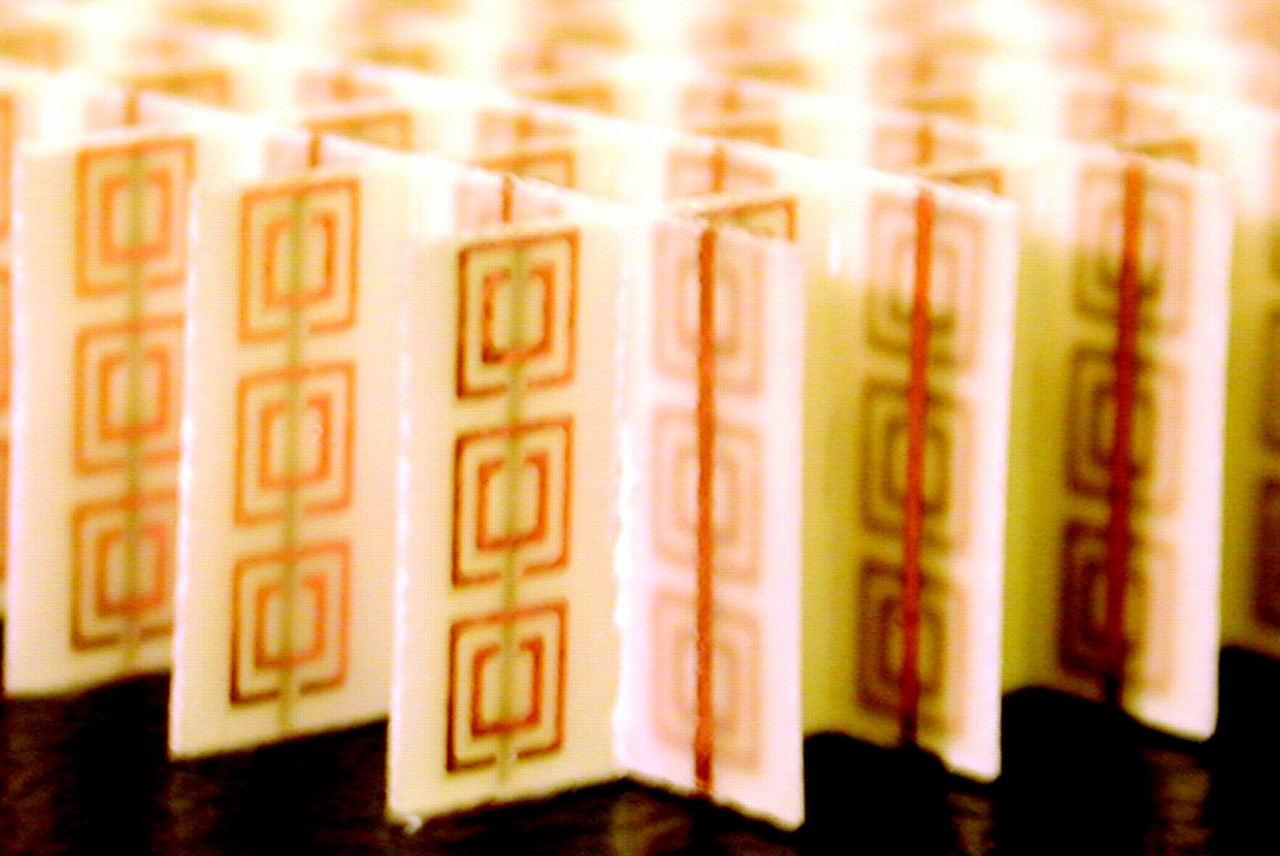
\includegraphics[width=0.8\linewidth]{sl_uvod/mm_smit.jpg}
    \caption{Експериментална реализација метаматеријала са негативними индексом~\cite{smith:00}.}
    \label{uvod:mm_smit}
\end{figure}
Прошло је више од тридесет година од Веселагове теоријске спекулације до реализације негативног индекса помоћу метаматеријала. Историјски, коришћење периодичних структура за синтезу диелектричне константе у микроталасној техници датира из педесетих година прошлог века, када су биле познате под термином „вештачки диелектрици`` (\foreign{artificial dielectric})~\cite{rotman1962plasma}. Пендри је предложио коришћење резонатора у облику прстена са процепом, тзв. сплит ринг резонатор, СРР (\foreign{split-ring, SRR}) за синтезу негативне пермеабилности~\cite{pendri:99}. Комбинацијом ова два приступа, фабриковани су метаматеријали који испољавају негативни индекс преламања у микроталасном опсегу~\cite{smith:00}.

Метаматеријал $<=>$ негативни индекс? Можда нешто рећи о томе докле су стигли са свим будалаштинама?

\section{Водови}

\bibliographystyle{babplai3}
\bibliography{ref}

\end{document}
